\documentclass[12pt]{article}
\usepackage{titling}
\usepackage{color}
\usepackage{float}
\usepackage{graphicx}
\graphicspath{ {images/} }
\usepackage{tikz}
\usetikzlibrary{arrows}


\newcommand{\todo}[1]{{\color{red}\ TODO: {#1}}}

\setlength{\droptitle}{-12em}
\title{Payment Subnetworks\vspace{-4.5em}}
\date{}
\author{}

\begin{document}
\maketitle
\begin{abstract}
Two-party duplex payment channels have been designed and linked together to construct payment networks to allow payment routing between parties that are not directly connected. A problem that members of this architecture might face is the need to rebalance ledgers. Enabling a set of nodes connected by payment channels to rebalance their ledgers off-chain would alleviate this issue. Implementation of this concept on the Ethereum blockchain rather than on Bitcoin can greatly simplify the model and amend its possible functionality.
\end{abstract}

\section{Introduction}
Off-chain payment protocols, such as the lightning \cite{lightning} and raiden \cite{raiden} networks, allow to move the burden of transaction settling from the blockchain to the two or more participating peers. 

Several new proposals have surfaced the literature that aim to improve the worst-case completion time of an off-chain transaction, such as in \cite{sprites}, or the scalability of blockchain payments, as in \cite{scale}.

The main contribution of this work is a ledger rebalancing scheme that enables each participant in the rebalancing to specify the amount of credit that they would like to gain or lose in each channel. The result of the scheme is a set of transactions that that need to be executed to carry out the rebalancing. We then enable the atomic execution of the set of payments on Ethereum using the Sprites payment channels \cite{sprites}, extending their atomic linked-payments functionality to a more general atomic payment-set functionality.

%The main contributions of this work are as follows:\vspace{-0.9em}
%\begin{itemize}
%	\item We incorporate the Sprites channels as a building unit of a hierarchy of multi-party subnetworks.
%	\item We integrate these subnetworks within global payment networks.
%	\item We create a ledger rebalancing scheme for subnetworks.
%\end{itemize}

\section{Background}
\todo{Explain high level concepts of what these technologies provide.}

\subsection{Bitcoin}
\todo{write overview of bitcoin for completeness in the future} \cite{bitcoin}
\subsection{Lightning}
The Bitcoin Lightning Network\cite{lightning} is an architecture that is designed to enable participants in the protocol to conduct a high volume of transactions in a secure manner without having to publish all of them to the Bitcoin blockchain.

The network is designed to be composed of peer-to-peer micropayment channels that enable two directly connected peers to maintain and use a shared ledger to securely conduct transactions, or for two indirectly connected peers to perform a transaction through a chain of directly connected intermediaries.

For a channel to be established between two entities, initial deposits representing the total amounts that can be transacted in this channel have to be put on the blockchain in escrow. The security lies in the assurance that in case of a dispute of payment or a need to withdraw deposits, the latest state of the ledger that the parties have agreed upon can be submitted to the blockchain and each party can claim its balance.

This design uses the bitcoin blockchain as a root of trust that would act upon an escrow account, and scales the blockchain essentially through aggregating transactions between parties that interact often, enabling high interaction throughputs without incurring the costs of on-chain publishing.

\subsection{Ethereum}
\todo{write overview of ethereum for completeness in the future} \cite{ethereum}

\subsection{Raiden}
The Raiden Network\cite{raiden} is a work in progress that aims to implement the same concepts proposed in the Lightning Network design, but on the Ethereum blockchain using smart contracts. Transaction costs are estimated to be 7 orders of magnitude lower using Raiden than natively on the blockchain, which would pave the way for efficient micropayments.

The project is as of now open-source, and has released a working proof of concept software version. However, Raiden has not yet been fully documented as to formally describe its techniques and functionality, but promises to deliver high scalability in the range of a million transactions per second, and transaction completion within a fraction of a second.

Because the Ethereum blockchain supports the creation of custom exchangeable tokens, the Raiden protocol aims to deliver the ability to make off-chain transactions with any token that follows the standard token API\cite{ethereum}.

\todo{Ask Raiden developers if they have some hidden white paper}


\subsection{Sprites}
Sprites\cite{sprites} are payment channels designed for Ethereum. Their design is also inspired by Lightning and Raiden, but they aim to minimize the worst-case collateral costs of indirect off-chain payments. Collateral cost is calculated as the amount of time funds are frozen, or held in escrow, instead of being utilized or invested, multiplied by the amount of money that is suspended from use.

When performing a linked payment
\footnote{An indirect off-chain payment using intermediaries that are directly "linked"}
the amount of money that is to be transacted has to be frozen across the entire chain of payment channels involved, until the transaction completes or terminates. This requirement is present in Lightning, Raiden and Sprites.

However, the achieved worst case time that a linked payment needs to complete or cancel in Sprites is not proportional to the length of the chain of intermediaries used to execute the payment, but is instead constant, unlike in Lightning and Sprites.

Since the total funds held in escrow during a linked payment using Sprites is proportional to the length of the transaction chain, and the upper bound on the amount of time is constant, the worst case collateral cost per payment that is only linearly, rather than quadratically\footnote{as in Lightning and Raiden}, proportional to the length of the chain used.

The innovative use of the turing complete smart contracts model offered by Ethereum to implement the payment channel concept, rather than the direct migration of an architecture meant for Bitcoin's limited UTXO
\footnote{Unspent Transaction Output}
model over to Ethereum, is what enables Sprites to provide its cost optimization.

\subsection{Channel Factories}
\cite{scale} proposes a design for Bitcoin whereby a group of parties announces the creation of a Channel Factory on the blockchain. When announcing the creation of this factory, its members first have to deposit their respective funds into a shared escrow account. They can then use their deposits in this on-chain escrow to fund the creation of off-chain escrow accounts between peers to create as many payment channels as needed off-chain.

For a party to join or depart a Channel Factory, however, a new on-chain factory has to be announced, where the deposits are transferred from the old factory's escrow account, and member balances are updated accordingly. In these entry and exit cases, all members of the Channel Factory have to approve and sign the aforementioned modifications.

An advantage that this construct has is that it allows the off-chain redistribution of deposits in the main escrow account of the Channel Factory between different payment channels constructed by the factory. Other designs require that any deposit to, or withdrawal of funds from, a payment channel escrow account happen purely on-chain, while in this design, only transactions with the main escrow account need to happen on-chain.

Essentially, this design enables the secure creation of off-chain m-out-of-m multisig wallets that are funded through one on-chain n-out-of-n multisig wallet, where the m participants in an off-chain wallet are a subset of the n participats of the on-chain wallet.

\todo{Mention scalability and expectations}

\section{Fundamental differences between Bitcoin and Ethereum}
\todo{Ethereum has smart contracts, Bitcoin has UTXO, etc.. highlight difference in functionality potential}

\section{Rebalancing Scheme}

\begin{figure}[H]
\centering
\begin{tikzpicture}[->,>=stealth',shorten >=1pt,auto,node distance=4cm,
                    thick,main node/.style={circle,draw,font=\sffamily\Large\bfseries}]

  \node[main node] (A) {A};
  \node[main node] (B) [right of=A] {B};
  \node[main node] (C) [below of=B] {C};
  \node[main node] (D) [below of=A] {D};

  \draw[-, every node/.style={font=\sffamily\small}]
  	(A) edge node[near start] {250}
  			 node[near end] {750} (B)
  		edge node[right, very near start] {750}
  			 node[left, very near end] {250} (C)
  		edge node[left, near start] {0}
  			 node[left, near end] {1000} (D)
  	(B) edge node[near start] {100}
  			 node[near end] {800} (C)
  		edge node[right, near start] {150}
  			 node[left, near end] {0} (D)
  	(C) edge node[near start] {750}
  		 	 node[near end] {0} (D)
  	;
\end{tikzpicture}
\caption{Example skewed network}
\label{skewed}
\end{figure}

A skewed network which might wish to rebalance its ledgers is presented in figure \ref{skewed}.

\subsection{Cooperative specification of rebalancing requirements}
Participants specify the maximum balance they wish to gain or lose in each channel, while preserving their total balance and not exceeding channel funds. We denote the maximum balance shift that a node u is willing to sustain in its payment channel with a node v by $\Delta_{u,v}$, additionally when using a directional arrow, $\overrightarrow{\Delta_{u,v}} = X$ signifies that u is willing to lose a balance of X in the u-v payment channel.

\subsection{Generation of rebalancing transaction set}
There are two independent approaches, with different flexibilities.

\textbf{Variant 1} Maximize a linear function in O(N) variables subject to O(N) linear inequality constraints. (N is the number of payment channels.)

Maximize: $\Sigma_{u,v} \delta_{u,v}$ (Total transacted funds) subject to:

\begin{enumerate}
	\item $\forall u, v: \Delta_{u,v} > 0 \wedge \Delta_{v,u} < 0 \Leftrightarrow 0 \leq \delta_{u,v} \leq min(\Delta_{u,v}, -\Delta_{v,u}) $

	\item $\forall u: \Sigma_{v} \delta_{v,u} = \Sigma_{v} \delta_{u,v} $
	
\end{enumerate}

The first constraint definition introduces linear constraints on the program when two parties connected by a payment channel agree on the flow of payment that they are willing to have in the channel. If A wishes to dispose of balance in the AB channel, and B wishes to gain balance in the same channel, then the $\delta_{a,b}$ parameter is given an upper bound.

The second constraint defines conservation of balance, such that the set of resulting transactions is a zero sum rebalance. It is assumed that $\Delta_{u,v} \leq bal_{u,v}$ for all inputs $\Delta_{u,v}$ such that no payment channel is used past its total funding.


This variant allows participants to specify for each payment channel that they are either willing to gain or lose up to a specific balance, but not both.


\textbf{Variant 2} Maximize a convex quadtratic function in O(N) variables subject to O(N) linear inequality constraints. (N is the number of payment channels.)

Maximize: $\Sigma_{u,v} \delta_{u,v}^2$ (Sum of squares of transacted funds) subject to:

\begin{enumerate}
	\item $\forall u, v: \delta_{u,v} = -\delta_{v,u}$

	\item $\forall u, v: \delta_{u,v} \leq min(\overrightarrow{\Delta_{u,v}},\overleftarrow{\Delta_{v,u}})$ 

	\item $\Sigma_{u,v} \delta_{u,v} = 0$
\end{enumerate}

The first constraint definition introduces the symmetry between $\delta_{u,v}$ and $\delta_{v,u}$, whereas in the previous model, only one of the two was ever present. This gives us more flexibility in the second constraint definition, which specifies that funds flowing in a direction across a payment channel must obey the both the upper and lower bounds set by the channel owners for each direction. This means that participants can specify how much balance they are willing to gain, and how much they are willing to lose, in a given channel, at the same time. This comes at the cost of having to solve for a convex quadratic function instead of a linear one. The third definition conserves balance.

\subsection{Rebalancing Protocol}

The protocol steps broadly defined in figure \ref{protocol} describe how the set of transactions is designed to either all atomically complete or fail.

\begin{figure}[H]
\centering
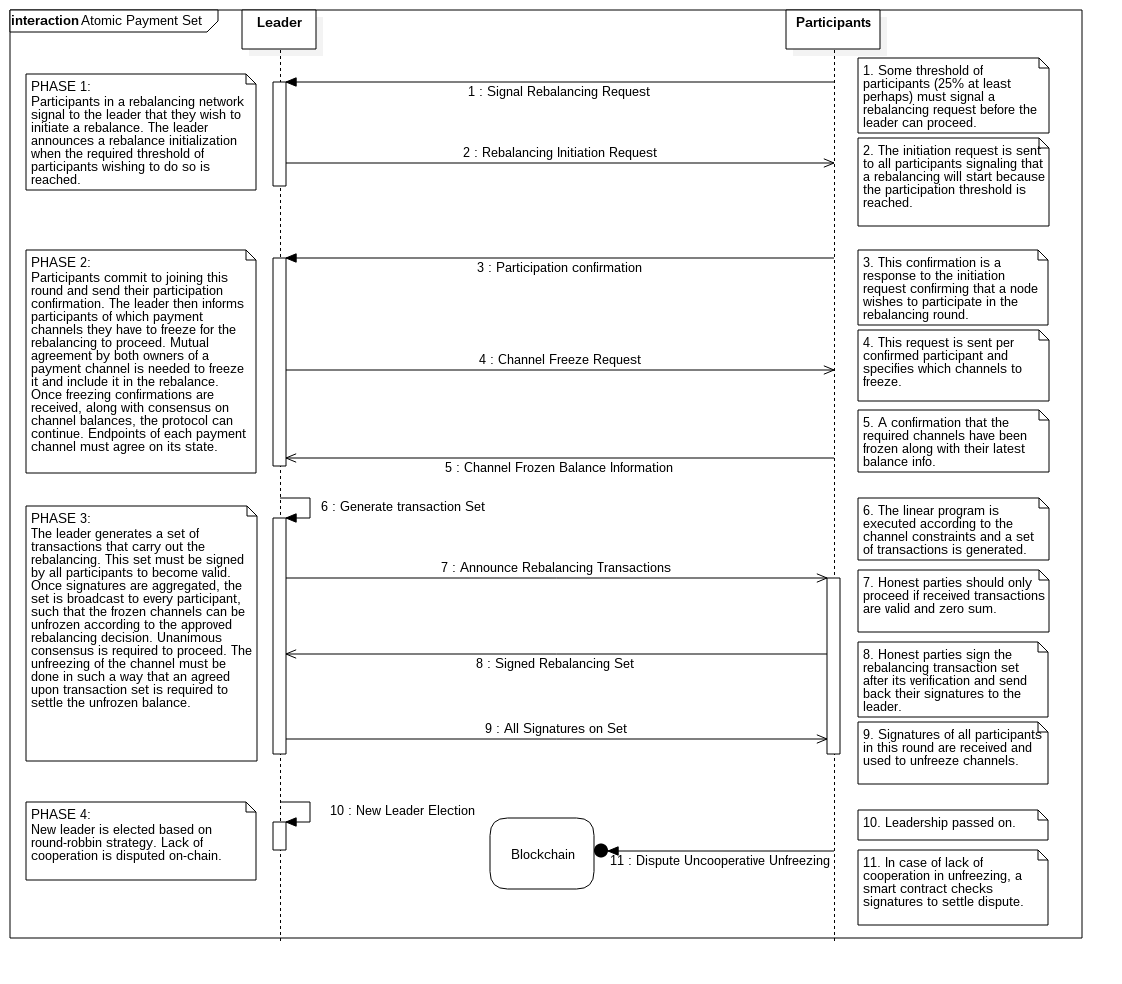
\includegraphics[width=\textwidth]{protocol}
\caption{Rebalancing Protocol}
\label{protocol}
\end{figure}

The set of payments is composed of multiple single conditional payments. The payments may only complete when the signatures of all participants in the rebalancing can be obtained on the payment set.

At first, the current elected leader waits for rebalancing initiation requests from participants in the subnetwork. When enough requests are received (past an arbitrarily defined threshold), then the leader sends a request to all subnet members which asks for confirmation of their participation in this round of rebalancing.

After participation confirmations are received, the leader then multi-casts to the participants which nodes will participate in the current round, and asks them to freeze the payment channels they wish to involve in this rebalancing round with a conditional payment, of an undetermined amount, that may only complete when all subnetwork members sign the set of transactions which the leader will propose in the next step.

After participants freeze their payment channels, and send confirmation of this to the leader node, the leader then proceeds to solve the linear program described above to generate a set of rebalancing transactions. The set is then sent to all nodes for verification and signing.

Once all signatures are obtained, they are multicast to all participants, such that they can unfreeze the payment channels. Any lack of cooperation in this step between parties can be disputed on chain through submission of the (mutually agreed upon) channel freezing confirmation and the unanimously signed payment set.

A new leader is then chosen via round-robin selection.

%\section{Channel Factories in Ethereum}

%The design of Channel Factories for Bitcoin proposes using expiring commitments or revocable transactions to proceed with off-chain payments. A design for Ethereum can make use of signatures and round numbers to simplify off-chain interactions and dispute settlement.

%\todo{Make diagrams to better illustrate following paragraph}

%The collaboration between stakeholders of a commitment of funds, however, when an operation that affects the redistribution of deposits needs to occur, cannot be circumvented or more efficiently designed. This means that when new members need to join a payment factory with a deposit, all current members must sign off on the new redistribution of deposits that occurs. Moreover, any ledger rebalancing which involves moving deposits across payment channels would require unanimous approval by the stake holders.

%\section{Combining Payment Subnets and Payment Networks}

%The details of integration of payment subnets within linked payment networks have not been discussed. For example: a linked payment whereby some of the intermediaries in the chain are both members of the same payment subnet, and would like to use their channel in this subnet as a link in the chain.

%An algorithm for subnet ledger rebalancing was not presented. Viewing a payment channel subnetwork constructed by a Channel Factory as a graph: An edge represents the shared ledger between two nodes in the subnet. An algorithm which rebalances ledgers in a way that satisfies the local preferences of each node in the network (ie. lets nodes assign ratios to their edges, such that their total balances are distributed across their edges according to these ratios), would be a point of interest after the construction of the subnet model.

\section{Related Work}
\section{Conclusion}

\bibliography{references}
\bibliographystyle{unsrt}

\end{document}
